\documentclass[10pt]{article}
\usepackage{../pplmanual}
\NeedsTeXFormat{LaTeX2e}
\typeout{^^J^^J
Parallel Programming Laboratory^^J
Manual Style^^J
Written by Milind A. Bhandarkar, 12/00^^J}

%%% Make it possible for both ps and pdf to be generated
\newif\ifpdf
\ifx\pdfoutput\undefined
  \pdffalse
\else
  \pdfoutput=1
  \pdftrue
\fi

\ifpdf
  \pdfcompresslevel=9
\fi

%%% Imported from fullpage.sty, since it is not always available
\topmargin 0pt
\advance \topmargin by -\headheight
\advance \topmargin by -\headsep

\textheight 8.9in

\oddsidemargin 0pt
\evensidemargin \oddsidemargin
\marginparwidth 1.0in

\textwidth 6.5in
%%% end import from fullpage

%%% Commonly Needed packages
\usepackage{graphicx,color,calc}
\usepackage{makeidx}
\usepackage{alltt}

%%% Commands for uniform looks of C++, Charm++, and Projections
\newcommand{\CC}{C\kern -0.0em\raise 0.5ex\hbox{\normalsize++}}
\newcommand{\emCC}{C\kern -0.0em\raise 0.4ex\hbox{\normalsize\em++}}
\newcommand{\charmpp}{\sc Charm++}
\newcommand{\projections}{\sc Projections}
\newcommand{\converse}{\sc Converse}
\newcommand{\ampi}{\sc AMPI}

%%% Commands to produce margin symbols
\newcommand{\new}{\marginpar{\fbox{\bf$\mathcal{NEW}$}}}
\newcommand{\important}{\marginpar{\fbox{\bf\Huge !}}}
\newcommand{\experimental}{\marginpar{\fbox{\bf\Huge $\beta$}}}

%%% Commands for manual elements
\newcommand{\zap}[1]{ }
\newcommand{\function}[1]{{\noindent{\textsf{#1}}\\}}
\newcommand{\cmd}[1]{{\noindent{\textsf{#1}}\\}}
\newcommand{\args}[1]{\hspace*{2em}{\texttt{#1}}\\}
\newcommand{\param}[1]{{\texttt{#1}}}
\newcommand{\kw}[1]{{\textsf{#1}}}
\newcommand{\uw}[1]{{\textsl{#1}}}
\newcommand{\desc}[1]{\indent{#1}}

%%% Commands needed for Maketitle
\newcommand{\@version}{}
\newcommand{\@credits}{}
\newcommand{\version}[1]{\renewcommand{\@version}{#1}}
\newcommand{\credits}[1]{\renewcommand{\@credits}{#1}}

%%% Print the License Page
\newcommand{\@license}{%
 \begin{center}
   {University of Illinois}\\
   {\charmpp/\converse\ Parallel Programming System Software}\\
   {Non-Exclusive, Non-Commercial Use License}\\
 \end{center}
 \rule{\textwidth}{1pt}
{\tiny
Upon execution of this Agreement by the party identified below (``Licensee''),
The Board of Trustees of the University of Illinois  (``Illinois''), on behalf
of The Parallel Programming Laboratory (``PPL'') in the Department of Computer
Science, will provide the \charmpp/\converse\ Parallel Programming System
software (``\charmpp'') in Binary Code and/or Source Code form (``Software'')
to Licensee, subject to the following terms and conditions. For purposes of
this Agreement, Binary Code is the compiled code, which is ready to run on
Licensee's computer.  Source code consists of a set of files which contain the
actual program commands that are compiled to form the Binary Code.

\begin{enumerate}
  \item
    The Software is intellectual property owned by Illinois, and all right,
title and interest, including copyright, remain with Illinois.  Illinois
grants, and Licensee hereby accepts, a restricted, non-exclusive,
non-transferable license to use the Software for academic, research and
internal business purposes only, e.g. not for commercial use (see Clause 7
below), without a fee.

  \item 
    Licensee may, at its own expense, create and freely distribute
complimentary works that interoperate with the Software, directing others to
the PPL server (\texttt{http://charm.cs.uiuc.edu}) to license and obtain the
Software itself. Licensee may, at its own expense, modify the Software to make
derivative works.  Except as explicitly provided below, this License shall
apply to any derivative work as it does to the original Software distributed by
Illinois.  Any derivative work should be clearly marked and renamed to notify
users that it is a modified version and not the original Software distributed
by Illinois.  Licensee agrees to reproduce the copyright notice and other
proprietary markings on any derivative work and to include in the documentation
of such work the acknowledgement:

\begin{quote}
``This software includes code developed by the Parallel Programming Laboratory
in the Department of Computer Science at the University of Illinois at
Urbana-Champaign.''
\end{quote}

Licensee may redistribute without restriction works with up to 1/2 of their
non-comment source code derived from at most 1/10 of the non-comment source
code developed by Illinois and contained in the Software, provided that the
above directions for notice and acknowledgement are observed.  Any other
distribution of the Software or any derivative work requires a separate license
with Illinois.  Licensee may contact Illinois (\texttt{kale@cs.uiuc.edu}) to
negotiate an appropriate license for such distribution.

  \item
    Except as expressly set forth in this Agreement, THIS SOFTWARE IS PROVIDED
``AS IS'' AND ILLINOIS MAKES NO REPRESENTATIONS AND EXTENDS NO WARRANTIES OF
ANY KIND, EITHER EXPRESS OR IMPLIED, INCLUDING BUT NOT LIMITED TO WARRANTIES OR
MERCHANTABILITY OR FITNESS FOR A PARTICULAR PURPOSE, OR THAT THE USE OF THE
SOFTWARE WILL NOT INFRINGE ANY PATENT, TRADEMARK, OR OTHER RIGHTS.  LICENSEE
ASSUMES THE ENTIRE RISK AS TO THE RESULTS AND PERFORMANCE OF THE SOFTWARE
AND/OR ASSOCIATED MATERIALS.  LICENSEE AGREES THAT UNIVERSITY SHALL NOT BE HELD
LIABLE FOR ANY DIRECT, INDIRECT, CONSEQUENTIAL, OR INCIDENTAL DAMAGES WITH
RESPECT TO ANY CLAIM BY LICENSEE OR ANY THIRD PARTY ON ACCOUNT OF OR ARISING
FROM THIS AGREEMENT OR USE OF THE SOFTWARE AND/OR ASSOCIATED MATERIALS.

  \item 
    Licensee understands the Software is proprietary to Illinois. Licensee
agrees to take all reasonable steps to insure that the Software is  protected
and secured from unauthorized disclosure, use, or release and  will treat it
with at least the same level of care as Licensee would use to  protect and
secure its own proprietary computer programs and/or information, but using no
less than a reasonable standard of care.  Licensee agrees to provide the
Software only to any other person or entity who has registered with Illinois.
If licensee is not registering as an individual but as an institution or
corporation each member of the institution or corporation who has access to or
uses Software must agree to and abide by the terms of this license. If Licensee
becomes aware of any unauthorized licensing, copying or use of the Software,
Licensee shall promptly notify Illinois in writing. Licensee expressly agrees
to use the Software only in the manner and for the specific uses authorized in
this Agreement.

  \item
    By using or copying this Software, Licensee agrees to abide by the
copyright law and all other applicable laws of the U.S. including, but not
limited to, export control laws and the terms of this license. Illinois  shall
have the right to terminate this license immediately by written  notice upon
Licensee's breach of, or non-compliance with, any terms of the license.
Licensee may be held legally responsible for any  copyright infringement that
is caused or encouraged by its failure to  abide by the terms of this license.
Upon termination, Licensee agrees to  destroy all copies of the Software in its
possession and to verify such  destruction in writing.

  \item
  The user agrees that any reports or published results obtained with  the
Software will acknowledge its use by the appropriate citation as  follows:

\begin{quote}
``\charmpp/\converse\ was developed by the Parallel Programming Laboratory in
the Department of Computer Science at the University of  Illinois at
Urbana-Champaign.''
\end{quote}

Any published work which utilizes \charmpp\ shall include the following
reference:

\begin{quote}
``L. V. Kale and S. Krishnan. \charmpp: Parallel Programming with Message-Driven
Objects. In 'Parallel Programming using \CC' (Eds. Gregory V. Wilson and Paul
Lu), pp 175-213, MIT Press, 1996.''
\end{quote}

Any published work which utilizes \converse\ shall include the following
reference:

\begin{quote}
``L. V. Kale, Milind Bhandarkar, Narain Jagathesan, Sanjeev Krishnan and Joshua
Yelon. \converse: An Interoperable Framework for Parallel Programming.
Proceedings of the 10th International Parallel Processing Symposium, pp
212-217, April 1996.''
\end{quote}

Electronic documents will include a direct link to the official \charmpp\ page
at \texttt{http://charm.cs.uiuc.edu/}

  \item
    Commercial use of the Software, or derivative works based thereon,
REQUIRES A COMMERCIAL LICENSE.  Should Licensee wish to make commercial use of
the Software, Licensee will contact Illinois (kale@cs.uiuc.edu) to negotiate an
appropriate license for such use. Commercial use includes: 

    \begin{enumerate}
      \item
	integration of all or part of the Software into a product for sale,
lease or license by or on behalf of Licensee to third parties, or 

      \item
	distribution of the Software to third parties that need it to
commercialize product sold or licensed by or on behalf of Licensee.
    \end{enumerate}

  \item
    Government Rights. Because substantial governmental funds have been  used
in the development of \charmpp/\converse, any possession, use or sublicense of
the Software by or to the United States government shall be subject to such
required restrictions.

  \item
    \charmpp/\converse\ is being distributed as a research and teaching tool
and as such, PPL encourages contributions from users of the code that might, at
Illinois' sole discretion, be used or incorporated to make the basic  operating
framework of the Software a more stable, flexible, and/or useful  product.
Licensees who contribute their code to become an internal  portion of the
Software agree that such code may be distributed by  Illinois under the terms
of this License and may be required to sign an  ``Agreement Regarding
Contributory Code for \charmpp/\converse\ Software'' before Illinois  can
accept it (contact \texttt{kale@cs.uiuc.edu} for a copy).
\end{enumerate}

UNDERSTOOD AND AGREED.

Contact Information:

The best contact path for licensing issues is by e-mail to
\texttt{kale@cs.uiuc.edu} or send correspondence to:

\begin{quote}
Prof. L. V. Kale\\
Dept. of Computer Science\\
University of Illinois\\
1304 W. Springfield Ave\\
Urbana, Illinois 61801 USA\\
FAX: (217) 333-3501
\end{quote}
}%tiny
 \newpage
}% end of license

\renewcommand{\maketitle}{\begin{titlepage}%
 \begin{flushright}
   {\Large
     Parallel Programming Laboratory\\
     University of Illinois at Urbana-Champaign\\
   }
 \end{flushright}
 \rule{\textwidth}{3pt}
 \vspace{\fill}
 \begin{flushright}
   \textsf{\Huge \@title \\}
 \end{flushright}
 \vspace{\fill}
 \@credits \\
 \rule{\textwidth}{3pt}
 \begin{flushright}
   {\large Version \@version}
 \end{flushright}
 \end{titlepage}
 \@license

 \tableofcontents
 \newpage
}% maketitle



\makeindex

\title{\charmpp\\ Finite Element Framework\\ Manual}
\version{1.2}
\credits{
Initial version of \charmpp{} Finite Element Framework was developed
by Milind Bhandarkar with inputs from Timothy Hinrichs and Karthikeyan
Mahesh. The current version is almost completely rewritten by
Orion Lawlor.
}

\begin{document}

\maketitle

\section{Introduction}

The Finite Element Method (FEM) approach is used in many engineering
applications with irregular domains, from elastic deformation problems to
crack propagation to fluid flow.  \charmpp{} is a free message-passing parallel
runtime system for machines from clusters of workstations to tightly-coupled
SMPs.  The \charmpp{} FEM framework allows you to write a parallel FEM program,
in C or Fortran 90, that closely resembles a serial version but includes
a few framework calls.

Using the FEM framework also allows you to take advantage of all the
features of \charmpp, including run-time load balancing,  performance
monitoring and visualization, and checkpoint/restart, with no additional
effort. The FEM framework also combines naturally with other \charmpp
frameworks built on TCHARM.

\subsection{Philosophy}

The \charmpp{} FEM framework is designed to be flexible, in that it
provided a few very general operations, such as loading and partitioning 
a ``mesh.''  
In describing these operations, we draw on examples from structural analysis,
but in fact the same calls can be used for other applications, including
fluid dynamics or partial differential equations solvers, or
even general-purpose graph manipulation.

For example, the FEM framework does not specify the number of spatial
dimensions.  Node locations are treated as just another kind of node data,
with no restrictions on the number of data items.
This allows the FEM framework to work with problems having any number 
of spatial dimensions.


\subsection{Terminology}

A FEM program manipulates elements and nodes. An \term{element} is a portion of
the problem domain, also known as a cell, and is typically some simple shape 
like a triangle, square, or hexagon in 2D; or tetrahedron or rectangular solid in 3D.  
A \term{node} is a point in the domain, and is often the vertex of several elements.  
Together, the elements and nodes form a \term{mesh}, which is the 
central data structure in the FEM framework.

An element knows which nodes surround it via the element's
\term{connectivity table}, which lists the nodes adjacent to each element.

\begin{figure}[h]
\begin{center}
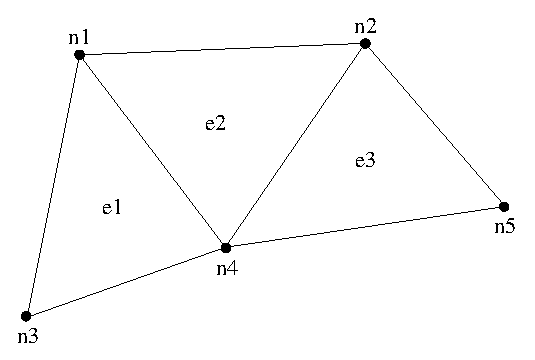
\includegraphics[width=4in]{fig/simple_mesh}
\end{center}
\caption{3-element, 5 node mesh.}
\label{fig:simplemesh}
\end{figure}

\begin{table}[h]
\begin{center}
\begin{tabular}{||l||l|l|l||}\hline
Element & \multicolumn{3}{c||}{Adjacent Nodes} \\\hline
e1 & n1 & n3 & n4 \\
e2 & n1 & n2 & n4 \\
e3 & n2 & n4 & n5 \\
\hline
\end{tabular}
\end{center}
\caption{Connectivity table for mesh in figure~\ref{fig:simplemesh}.}
\label{table:simplemesh}
\end{table}

A typical FEM program performs some element-by-element calculations which
update adjacent node values; then some node-by-node calculations.  For
example, a material dynamics program has the structure:

\begin{alltt}
     time loop
          element loop-- Element deformation applies forces to
          surrounding nodes
          node loop-- Forces and boundary conditions change node
          positions
     end time loop
\end{alltt}

We can parallelize such FEM programs by partitioning the serial mesh
elements into several smaller meshes, or \term{chunks}.  There is normally
at least one chunk per processor; and often even more.  During partitioning, 
we give nodes and elements new, \term{local} numbers within that chunk.
In the figure below, we have partitioned the mesh above into two chunks, A and B.

\begin{figure}[h]
\begin{center}
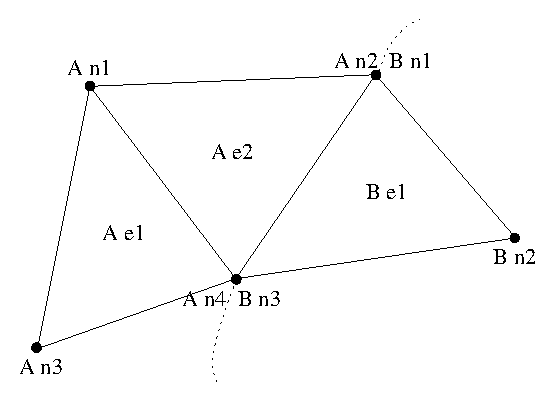
\includegraphics[width=4in]{fig/partitioned_mesh}
\end{center}
\caption{Partitioned mesh.}
\label{fig:partitionedmesh}
\end{figure}

\begin{table}[hh]
\begin{center}
\begin{tabular}{||l||l|l|l||}\hline
Element & \multicolumn{3}{c||}{Adjacent Nodes} \\\hline
e1 & n1 & n3 & n4 \\
e2 & n1 & n2 & n4 \\
\hline
\end{tabular}
\end{center}
\caption{Connectivity table for chunk A in figure~\ref{fig:partitionedmesh}.}
\label{table:chunkA}
\end{table}

\begin{table}[hh]
\begin{center}
\begin{tabular}{||l||l|l|l||}\hline
Element & \multicolumn{3}{c||}{Adjacent Nodes}\\\hline
e1 & n1 & n2 & n3 \\
\hline
\end{tabular}
\end{center}
\caption{Connectivity table for chunk B in figure~\ref{fig:partitionedmesh}.}
\label{table:chunkB}
\end{table}

Note that chunk A's node n2 and B's node n1 were actually the same node in
the original mesh-- partitioning split this single node into two shared
copies (one on each chunk).  However, since adding forces is associative, we
can handle shared nodes by computing the forces normally (ignoring the
existence of the other chunk), then adding both chunks' net force for the
shared node together.  This ``node update'' will give us the same resulting
force on each shared node as we would get without partitioning, thus the
same positions, thus the same final result.  

For example, under hydrostatic pressure, each chunk might compute a local
net force vector for its nodes as shown in Figure~\ref{fig:forcedecomp}
(a).  After adding forces across chunks, we have the consistent global forces
shown in Figure~\ref{fig:forcedecomp} (b).

\begin{figure}[h]
\begin{center}
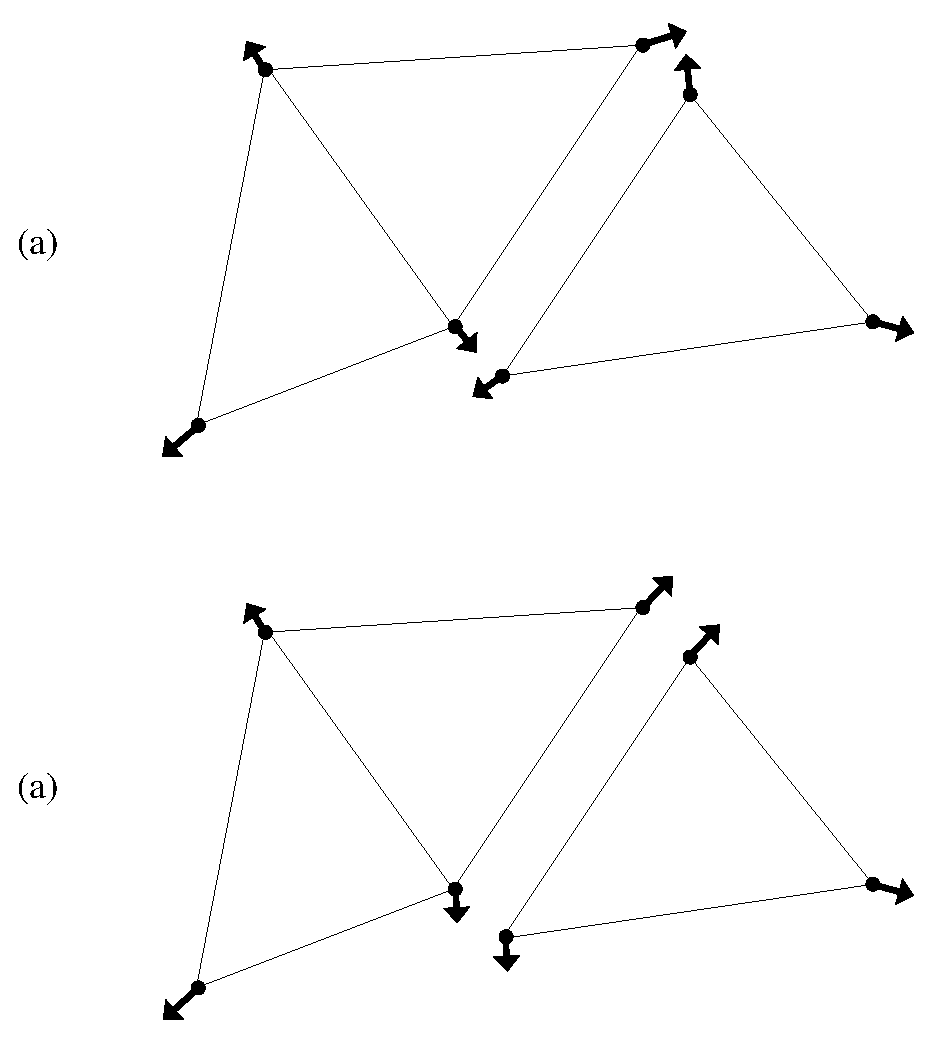
\includegraphics[height=3in]{fig/forcedecomp}
\end{center}
\caption{A force calculation decomposed across chunks: (a) before update
(b) after updating forces across nodes.}
\label{fig:forcedecomp}
\end{figure}

Hence, each chunk's time loop has the structure:

\begin{alltt}
     chunk time loop
          element loop-- Element deformation applies forces to
          surrounding nodes
          <update forces on shared nodes>
          node loop-- Forces and boundary conditions change node
          positions
     end time loop
\end{alltt}

This is exactly the form of the time loop for a \charmpp{} FEM framework
program.  The framework will accept a serial mesh, partition it, distribute
the chunks to each processor, allow the user to run their time loop, and
handle the node-updates.


\subsection{Structure of a FEM Framework Program}

A FEM framework program consists of two subroutines: \kw{init()} and \kw{driver()}.
\kw{init()} is called by the FEM framework
only on the first processor -- this routine typically does specialized I/O,
startup and shutdown tasks.  \kw{driver()} is called for every chunk on every
processor, and does the main work of the program.  In the language of the
TCHARM manual, \kw{init()} runs in the serial context, 
and \kw{driver()} runs in the parallel context.


\begin{alltt}
     subroutine init
          read the serial mesh and configuration data
     end subroutine

     subroutine driver
          get local mesh chunk
          time loop
               FEM computations
               update shared node fields
               more FEM computations
          end time loop
     end subroutine
\end{alltt}

\subsection{Compilation and Execution}

A FEM framework program is a \charmpp\ program, so you must begin by
downloading the latest source version of \charmpp\ from
{\tt http://charm.cs.uiuc.edu/}.  Build the source with 
{\tt ./build FEM version} or {\tt cd} into the build directory, 
{\tt version/tmp}, and type {\tt make FEM}.
To compile a FEM program, pass the {\tt -language fem} (for C) or 
{\tt -language femf} (for Fortran) option to {\tt charmc}.

In a charm installation, see charm/version/pgms/charm++/fem/
for several example and test programs.

At runtime, an FEM framework program accepts the following
options, in addition to all the usual Charm++ options described in 
the Charm++ ``Installation and Usage Manual''.

\begin{itemize}
\item {\tt +vp} $v$  

Create $v$ mesh chunks, or ``virtual processors''.
By default, the number of mesh chunks is equal to the number of 
physical processors (set with {\tt +p} $p$).


\item {\tt -write}

Skip \kw{driver()}.
After running \kw{init()} normally, the framework partitions the mesh, 
writes the mesh partitions to files, and exits.  As usual, the
{\tt +vp} $v$ option controls the number of mesh partitions.


\item {\tt -read}

Skip \kw{init()}.
The framework reads the partitioned input mesh from files
and calls \kw{driver()}.  Together with {\tt -write}, this option
allows you to separate out the mesh preparation and partitioning 
phase from the actual parallel solution run.

This can be useful, for example, if \kw{init()} requires more memory 
to hold the unpartitioned mesh than is available on one processor of 
the parallel machine.  To avoid this limitation, you can run the program
with {\tt -write} on a machine with a lot of memory to prepare the input
files, then copy the files and run with {\tt -read} on a machine with 
a lot of processors.

{\tt -read} can also be useful during debugging or performance tuning, 
by skipping the (potentially slow) mesh preparation phase.


\item {\tt +tcharm\_trace fem}

Give a diagnostic printout on every call into the FEM framework.
This can be useful for locating a sudden crash, or understanding
how the program and framework interact.  Because printing the 
diagnostics can slow a program down, use this option with care.

\end{itemize}


\section{FEM Framework API Reference}

Some of the routines in the FEM framework have different requirements or meanings
depending on where they are called from.  When a routine is described
as being ``called from driver'', this means it is called in the parallel
context---from \kw{driver()} itself, any subroutine called by \kw{driver()},
or from whatever routine is run by the FEM-attached TCHARM threads.
When a routine is described as being ``called from init'', this means it is 
called in the serial context---from \kw{init()} itself, from any subroutine
called from \kw{init()}, from a routine called by \kw{FEM\_Update\_mesh},
or from whatever TCHARM code executes before the \kw{FEM\_Attach}.


\subsection{Utility}

\prototype{FEM\_Num\_partitions}
\function{int FEM\_Num\_partitions();}
\function{function integer :: FEM\_Num\_partitions()}

     Return the number of mesh chunks in the current computation.  Can
     only be called from the driver routine.

\prototype{FEM\_My\_partitions}
\function{int FEM\_My\_partition();}
\function{function integer :: FEM\_My\_partition()}

     Return the number of the current chunk, from 0 to
     \kw{num\_partitions}-1.  Can only be called from the driver routine.

\prototype{FEM\_Timer}
\function{double FEM\_Timer();}
\function{function double precision :: FEM\_Timer()}

     Return the current wall clock time, in seconds.  Resolution is
     machine-dependent, but is at worst 10ms.

\prototype{FEM\_Print\_partition}
\function{void FEM\_Print\_partition();}
\function{subroutine FEM\_Print\_partition()}

     Print a debugging representation of the current chunk's mesh.
     Prints the entire connectivity array, and data associated with
     each local node and element.

\prototype{FEM\_Print}
\function{void FEM\_Print(const char *str);}
\function{subroutine FEM\_Print(str)}
\args{  character*, intent(in) :: str}

     Print the given string.  Works on all machines; unlike \kw{printf} or
     \kw{print *}, which may not work on all parallel machines.


{\it TERRY}

\subsection{Mesh Entities}
\label{sec:entities}

{\it TERRY}

\subsubsection{Nodes}
\label{sec:nodes}

{\it TERRY}

\subsubsection{Elements}
\label{sec:elements}

{\it TERRY}

\subsubsection{Sparse Elements}
\label{sec:sparse}

{\it TERRY}

\subsubsection{Mesh Entity Operations}

{\it TERRY}

\subsubsection{Mesh Entity Queries}

{\it TERRY}

\subsubsection{Advanced Mesh Entity Operations}

{\it TERRY}

\subsection{Meshes}
\label{sec:meshes}

{\it TERRY}

\subsubsection{Basic Mesh Operations}

{\it TERRY}

\subsubsection{Mesh Utilities}

{\it TERRY}

\subsubsection{Advanced Mesh Operations}

{\it TERRY}

\subsection{Mesh Communication: Ghost Layers}
\label{sec:ghost}

{\it SAYANTAN}

\subsubsection{Ghost Numbering}

{\it SAYANTAN}

\subsubsection{Ghost Layer Creation}

{\it SAYANTAN}

\subsubsection{Symmetries and Ghosts: Geometric Layer}

{\it SAYANTAN}

\subsubsection{Advanced Symmetries and Ghosts: Lower Layer}

{\it SAYANTAN}

\subsection{Older Mesh Operations}

{\it SAYANTAN}

\subsubsection{Mesh Data Operations}

{\it SAYANTAN}

\subsubsection{Ghost Numbering}

{\it SAYANTAN}

\subsubsection{Backward Compatability}

{\it SAYANTAN}

\subsubsection{Sparse Data}

{\it SAYANTAN}

\subsection{Mesh Modification}

{\it AARON}

\subsection{Topological Mesh Data}

{\it ISAAC}

\subsection{Mesh Adaptivity}


\subsubsection{Initialization}
If a ParFUM application wants to use parallel mesh adaptivity,
the first task is to call the initialization routine from the 
{\it driver} function. This creates the node and element 
adjacency information that is essential for the adaptivity 
operations. It also initializes all the mesh adaptivity related
internal objects in the framework.

\function{void FEM\_ADAPT\_Init(int meshID)}
\index{femAdaptInit}
\desc{Initializes the mesh defined by {\it meshID} for the mesh
adaptivity operations.}

\subsubsection{Preparing the Mesh}
For every element entity in the mesh, there is a desired size entry 
for each element. This entry is called meshSizing. This meshSizing entry 
contains a metric that determines element quality. The default metric is
the average of the length of the three edges of an element. ParFUM provides 
various mechanisms to set this field. Some of the adaptive operations
use these metrics to maintain quality. In addition, there is another metric
which is computed for each element and maintained during mesh adaptivity. This metric 
is the ratio of the longest side to the shortest altitude, and this value 
is not allowed to go beyond a certain limit in order to maintain element quality.

\function{void FEM\_ADAPT\_SetElementSizeField(int meshID, int elem, double size);}
\index{femAdaptSetElementSizeField1}
\desc{For the mesh specified by {\it meshID}, for the element {\it elem},
we set the desired size for each element to be {\it size}.}

\function{void FEM\_ADAPT\_SetElementSizeField(int meshID, double *sizes);}
\index{femAdaptSetElementSizeField2}
\desc{For the mesh specified by {\it meshID}, for the element {\it elem},
we set the desired size for each element from the corresonponding entry in
the {\it sizes} array.}

\function{void FEM\_ADAPT\_SetReferenceMesh(int meshID);}
\index{femAdaptSetReferenceMesh}
\desc{For each element int this mesh defined by {\it meshID} 
set its size to the average edge length of the corresponding element.}

\function{void FEM\_ADAPT\_GradateMesh(int meshID, double smoothness);}
\index{femAdaptGradateMesh}
\desc{Resize mesh elements to avoid jumps in element size.
That is, avoid discontinuities in the desired sizes for elements of a mesh
by smoothing them out. Algorithm based on h-shock correction, described in
Mesh Gradation Control, Borouchaki et al.}


\subsubsection{Modifying the Mesh}
Once the elements in the mesh have been prepared by specifying their desired
sizes, we are ready to use the actual adaptivity operations. Currently we
provide delaunay flip operations, edge bisect operations and edge coarsen 
operations, all of which are implemented in parallel. We provide several higher level 
functions which use these basic operations to 
generate a mesh with higher quality elements while achieving the
desired sizing.

\function{void FEM\_ADAPT\_Refine(int meshID, int qm, int method, double factor,double *sizes);}
\index{femAdaptRefine}
\desc{Perform refinements on the mesh specified by {\it meshId}.
Tries to maintain/improve element quality by refining the mesh
as specified by a quality measure {\it qm}.
If {\it method} = 0, refine areas with size larger than {\it factor} down to {\it factor}
If {\it method} = 1, refine elements down to sizes specified in the {\it sizes} array.
In this array each entry corresponds to the corresponding element.
Negative entries in sizes array indicate no refinement. }

\function{void FEM\_ADAPT\_Coarsen(int meshID, int qm, int method, double factor,double *sizes);}
\index{femAdaptCoarsen}
\desc{Perform refinements on the mesh specified by {\it meshId}.
Tries to maintain/improve element quality by coarsening the mesh
as specified by a quality measure {\it qm}.
If {\it method} = 0, coarsen areas with size smaller than {\it factor} down to {\it factor}
If {\it method} = 1, coarsen elements up to sizes specified in the {\it sizes} array.
In this array each entry corresponds to the corresponding element.
Negative entries in sizes array indicate no coarsening. }

\function{void FEM\_ADAPT\_AdaptMesh(int meshID, int qm, int method, double factor,double *sizes);}
\index{femAdaptAdaptMesh}
\desc{This function has the same set of arguments as required by the previous two operations,
namely refine and coarsen. This function keeps using the above two functions until
we have all elements in the mesh with as close to the desired quality. Apart from
using the above two operations, it also performs a mesh repair operation which
gets rid of some bad quality elements by delaunay flip or coarsening as the
geometry in the area demands.}

\function{int FEM\_ADAPT\_SimpleRefineMesh(int meshID, double targetA, double xmin, double ymin, double xmax, double ymax);}
\index{femAdaptSimpleRefineMesh}
\desc{A region is defined by ({\it xmax, xmin, ymax, ymin}) 
and the target area to be achieved for all elements in this region
in the mesh specified by {\it meshID} is given by {\it targetA}.
This function only performs a series of refinements on the elements in this region.
If the area is larger, then no coarsening is done.}

\function{int FEM\_ADAPT\_SimpleCoarsenMesh(int meshID, double targetA, double xmin, double ymin, double xmax, double ymax);}
\index{femAdaptSimpleCoarsenMesh}
\desc{A region is defined by ({\it xmax, xmin, ymax, ymin}) 
and the target area to be achieved for all elements in this region
in the mesh specified by {\it meshID} is given by {\it targetA}.
This function only performs a series of coarsenings on the elements in this region.
If the area is smaller, then no refinement is done.}


\subsection{Verifying correctness}
We provide a checking function that can be used for debugging purposes to identify corrupted meshes or low quality elements.

\function{void FEM\_ADAPT\_TestMesh(int meshID);}
\index{femAdaptTestMesh}
\desc{This provides a series of tests to determine the consistency of the
mesh specified by {\it meshID}.}


\section{IDXL Communication}

The FEM framework's communication layer is called IDXL. This small library handles sending and receiving data to and from a sparse subset of 1D indices into a user array.  The sparse index subset is called an "Index List", hence the name of the library.


\subsection{Index Lists}
\label{sec:IDXL}
An Index List is the fundamental data structure of the IDXL library---for example, the list of shared nodes is an Index List.  IDXL includes routines for building, combining, and sending and receiving Index Lists.

An Index List, as you might expect, is a list of indices that need to be sent and received.  An Index List includes both the indices that need to be sent, as well as the indices to be received, from each chunk.

Consider two chunks $a$ and $b$ where $b$ needs some information $a$ has, such as if $b$ has ghosts of real elements on $a$.  $a$'s Index List thus has a send portion with the $a$-local indices for the elements $a$ sends; and $b$'s Index List contains a receive portion with the $b$-local indices for the elements $b$ receives.  Thus across processors, the corresponding send and receive portions of $a$ and $b$'s Index Lists match, as shown in Figure~\ref{fig:indexlists}.


\begin{figure}[h]
\begin{center}
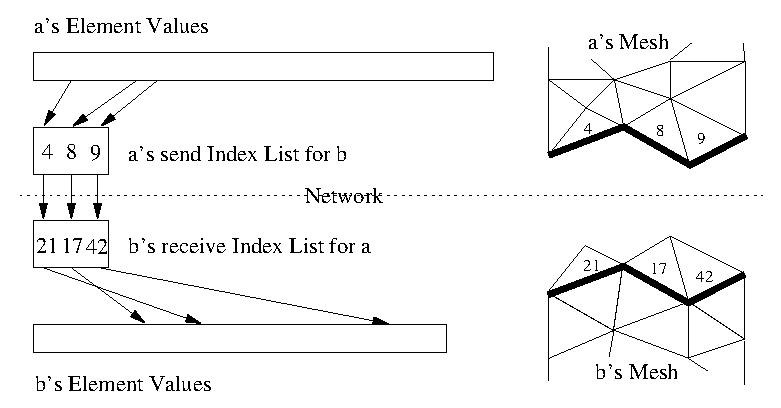
\includegraphics[width=5in]{fig/indexlists}
\end{center}
\caption{Illustrating how Index Lists match up $a$'s source elements with $b$'s ghost elements.}
\label{fig:indexlists}
\end{figure}



%%%%%%%%%%%%%%%%%%% Index Lists %%%%%%%%%%%%%%%%%%%%
\subsubsection{Index List Calls}

You refer to an Index List via an opaque handle---in C, the integer typedef \kw{IDXL\_t}; in Fortran, a bare INTEGER.  


\prototype{FEM\_Comm\_shared}
\function{IDXL\_t FEM\_Comm\_shared(int mesh,int entity);}
\function{INTEGER function FEM\_Comm\_shared(mesh,entity)}
  \args{INTEGER, INTENT(IN)  :: mesh,entity}

Return a read-only copy of the Index List of shared nodes.  The send and receive portions of this list are identical, because each shared node is both sent and received.  Shared nodes are most often used with the \kw{send/sum} communication pattern.

Must be called from driver.  \kw{mesh} must be a reading mesh. \kw{entity} must be \kw{FEM\_NODE}.  You may not call \kw{IDXL\_Destroy} on the returned list.


\prototype{FEM\_Comm\_ghost}
\function{IDXL\_t FEM\_Comm\_ghost(int mesh,int entity);}
\function{INTEGER function FEM\_Comm\_ghost(mesh,entity)}
  \args{INTEGER, INTENT(IN)  :: mesh,entity}

Return a read-only copy of the Index List of ghost entities.  The send portion of this list contains real, interior entities, which are sent away; the receive portion of the list contains the ghost entites, which are received. Ghosts are most often used with the \kw{send/recv} communication pattern.

Elements to be sent out are listed starting at zero (one in Fortran); but ghost elements to be received are also listed starting at zero (one in Fortran).  If real and ghost elements are kept in separate arrays, this is usable as-is; but if ghosts and real elements are kept together, you will need to shift the ghost indices using \kw{IDXL\_Combine} or \kw{IDXL\_Shift}. 

This routine must be called from driver.  \kw{mesh} must be a reading mesh. \kw{entity} must not include \kw{FEM\_GHOST}--ghosts are already included.  You may not call \kw{IDXL\_Destroy} on the returned list.


\prototype{IDXL\_Create}
\function{IDXL\_t IDXL\_Create(void);}
\function{INTEGER function IDXL\_Create()}

Create a new, empty Index List. This list can then be filled up using \kw{IDXL\_Copy} or \kw{IDXL\_Combine}.

Must be called from driver.  You must eventually call \kw{IDXL\_Destroy} on the returned list.


\prototype{IDXL\_Combine}
\function{void IDXL\_Combine(IDXL\_t dest,IDXL\_t src,int startSend,int startRecv);}
\function{SUBROUTINE IDXL\_Combine(dest,src,startSend,startRecv)}
  \args{INTEGER, INTENT(IN)  :: dest,src,startSend,startRecv}

Add the shifted contents of the src Index List to dest.  The send portion of src is shifted so the first index sent will be startSend; for a ghost index list this is the index of the first sent real entity. The receive portion of src is similarly shifted so the first index received will be startRecv; for a ghost index list this is the index of the first received ghost entity.  

This routine does not check for duplicates---if an index originally appears in dest and the also in the shifted src, it will be listed twice.


\subsubsection{Advanced Index List Calls}

\prototype{IDXL\_Destroy}
\function{void IDXL\_Destroy(IDXL\_t l);}
\function{SUBROUTINE IDXL\_Destroy(l)}
  \args{INTEGER, INTENT(IN)  :: l}

Destroy this Index List, and free the list storage allocated by the framework.  Only call this routine with lists you created using \kw{IDXL\_Create}; not lists obtained directly from the FEM framework.

\prototype{IDXL\_Print}
\function{void IDXL\_Print(IDXL\_t l);}
\function{SUBROUTINE IDXL\_Print(l)}
  \args{INTEGER, INTENT(IN)  :: l}

Print out the contents of this Index List.  This routine shows both the send and receive indices on the list, for each chunk we communicate with.


\prototype{IDXL\_Copy}
\function{void IDXL\_Copy(IDXL\_t dest,IDXL\_t src);}
\function{SUBROUTINE IDXL\_Print(dest,src)}
  \args{INTEGER, INTENT(IN)  :: dest,src}

Copy the contents of the source Index List into the destination Index List, which should be empty.

\prototype{IDXL\_Shift}
\function{void IDXL\_Shift(IDXL\_t l,int startSend,int startRecv);}
\function{SUBROUTINE IDXL\_Shift(l,startSend,startRecv)}
  \args{INTEGER, INTENT(IN)  :: l,startSend,startRecv}

Like \kw{IDXL\_Combine}, but only shifts the indices within a single list.


\prototype{IDXL\_Add\_entity}
\function{void IDXL\_Add\_entity(int newIdx,int nBetween,int *between);}
\function{SUBROUTINE IDXL\_Add\_node(newIdx,nBetween,between)}
    \args{INTEGER, INTENT(IN) :: newIdx,nBetween}
    \args{INTEGER, INTENT(IN) :: between(nBetween)}

This call adds a new entity, with local index \kw{newIdx}, to this Index List.  The new entity is sent or received by each chunk that sends or receives all the entities listed in the between array.  For example, when adding a new node along an edge, nBetween is 2 and between lists the endpoints of the edge; this way if the edge is shared with some chunk, the new node will be shared with that chunk.

This routine only affects the current chunk-- no other chunks are affected.  To ensure the communication lists match, \kw{IDXL\_Add\_entity} must be called on all the chunks that send or receive the entity, to create the local copies of the entity.

\kw{IDXL\_Add\_entity} adds the new entity to the end of the communication list, and so must be called in the same order on all the chunks that share the new entity.  For example, if two new nodes $x$ and $y$ are added between chunks $a$ and $b$, if chunk $a$ calls \kw{IDXL\_Add\_entity} with its local number for $x$ before it calls \kw{IDXL\_Add\_entity} with its local number for $y$, chunk $b$ must also add its copy of node $x$ before adding $y$.

% FIXME: implement, and document, IDXL\_Sort\_2d and IDXL\_Sort\_3d

%%%%%%%%%%%%%%%%%%% Layout %%%%%%%%%%%%%%%%%%%%
\subsection{Data Layout}
\label{sec:IDXLLayout}
IDXL is designed to send and receive data directly out of your arrays, with no intermediate copying.  This means IDXL needs a completely general method for specifying how you store your data in your arrays.  Since you probably don't change your storage layout at runtime, you can create a ``data layout'' once at the beginning of your program, then use it repeatedly for communication.

IDXL Layouts are normally used to describe arrays of data associated with nodes or elements.  The layout abstraction allows you to use IDXL routines to communicate any sort of data, stored in a variety of formats.

Like Index Lists, Layouts are referred to via an opaque handle---in a C program via the integer typedef IDXL\_Layout\_t, and in Fortran via a bare integer.

\subsubsection{Layout Routines}

In most programs, the data to be communicated is a dense array of data of one type.  In this case, there is only one layout routine you need to know:

\prototype{IDXL\_Layout\_create}
\function{IDXL\_Layout\_t IDXL\_Layout\_create(int type,int width);}
\function{INTEGER function IDXL\_Layout\_create(type,width)}
    \args{INTEGER, INTENT(IN) :: type,width}

The simplest data layout to describe---a dense array of this IDXL datatype, indexed by entity number, with \kw{width} pieces of data per entity. Note that the number of entities is not stored with the layout--the number of entities to be communicated depends on the communication routine.

The IDXL datatypes are:
\begin{center}
\begin{tabular}{|l|l|l|}\hline
IDXL Datatype & C Datatypes & Fortran Datatypes \\\hline
\kw{IDXL\_BYTE} & unsigned char & INTEGER*1 \\
               & char & LOGICAL*1 \\
\kw{IDXL\_INT} & int & INTEGER \\
\kw{IDXL\_REAL} & float & SINGLE PRECISION \\
                &  & REAL*4 \\
\kw{IDXL\_DOUBLE} & double & DOUBLE PRECISION \\
                  &  & REAL*8 \\
\hline
\end{tabular}
\end{center}

For example, if you keep a dense array with 3 doubles of force per node, you'd call this routine as:

\begin{alltt}
// C++ version:
     double *force=new double[3*n];
     IDXL\_Layout\_t force\_layout=IDXL\_Layout\_create(IDXL\_DOUBLE,3);

! F90 Version
     double precision, allocatable :: force(:,:)
     integer :: force\_layout
     ALLOCATE(force(3,n)) ! (could equivalently use force(3*n) )
     force\_layout=IDXL\_Layout\_create(IDXL\_DOUBLE,3)

\end{alltt}

This routine was once called \kw{FEM\_Create\_simple\_field}.


\subsubsection{Advanced Layout Routines}
\label{sec:IDXLLayoutoffset}

These advanced routines are only needed if you want to exchange data stored in an array of user-defined types.  Most programs only need \kw{IDXL\_Layout\_create}.

\prototype{IDXL\_Layout\_offset}
\function{IDXL\_Layout\_t IDXL\_Layout\_offset(int type, int width, int offsetBytes, int distanceBytes,int skewBytes);}
\function{INTEGER function IDXL\_Layout\_offset(type,width,offsetBytes,distanceBytes,skewBytes)}
    \args{INTEGER, INTENT(IN) :: type,width,offsetBytes,distanceBytes,skewBytes}

The most general data layout--an array indexed by entity, containing \kw{width} pieces of data per entity.  This routine expands on \kw{IDXL\_Layout\_create} by adding support for user-defined types or other unusual data layouts.  You describe your layout by giving various in-memory byte offsets that describe the data is stored. Again, the number of entities is not stored with the layout--the number of entities to be communicated depends on the communication routine.

\begin{itemize}
  \item \kw{offsetBytes} The number of bytes from the start of the array to the start of the data.
  \item \kw{distanceBytes} The number of bytes taken by one entity.
  \item \kw{skewBytes} The number of bytes between each piece of data.  Since this can almost always be determined from the size of the base data type, this parameter can be left as zero.
\end{itemize}

\begin{figure}[h]
\begin{center}
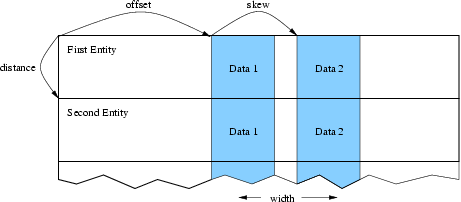
\includegraphics[width=5in]{fig/layout}
\end{center}
\caption{Describing a complex data layout.}
\label{fig:layout}
\end{figure}

For example, if your node data is all stored in a struct (in fortran, a named TYPE), offsetBytes gives the distance between the start of the struct and the force; and distanceBytes gives the size in bytes of the struct.  

In C, the offsetof and sizeof keywords are useful for finding these values.  In Fortran, we provide a special routine called \kw{foffsetof} that returns the distance, in bytes, between its two arguments.

\begin{alltt}
// C++ version:
     typedef struct \{
        double d[3], v[3], force[3], a[3];
        double m;
     \} node;
     node *nodes=new node[n];
     IDXL\_Layout\_t force\_layout=IDXL\_Layout\_offset(IDXL\_DOUBLE,3,
              offsetof(node,force),sizeof(node),0);

! F90 Version
     TYPE node 
        DOUBLE PRECISION :: d(3), v(3), force(3), a(3)
        DOUBLE PRECISION :: m
     END TYPE
     integer :: force\_layout
     ALLOCATE(nodes(n))
     force\_layout=IDXL\_Layout\_create(IDXL\_DOUBLE,3,
   &          foffsetof(nodes(1),nodes(1)\%force),
   &          foffsetof(nodes(1),nodes(2)),0)
\end{alltt}


\prototype{IDXL\_Layout\_destroy}
\function{void IDXL\_Layout\_destroy(IDXL\_Layout\_t layout);}
\function{SUBROUTINE IDXL\_Layout\_destroy(layout)}
  \args{INTEGER, INTENT(IN)  :: layout}

Destroy this Layout.  You only need call this routine if you repeatedly create layouts.

\prototype{IDXL\_Get\_layout\_type}
\function{int IDXL\_Get\_layout\_type(IDXL\_Layout\_t layout);}
\function{INTEGER function IDXL\_Get\_layout\_type(layout)}

Return the IDXL datatype for this layout.

\prototype{IDXL\_Get\_layout\_width}
\function{int IDXL\_Get\_layout\_width(IDXL\_Layout\_t layout);}
\function{INTEGER function IDXL\_Get\_layout\_width(layout)}

Return the layout width---the number of data items that are communicated
per entity.

\prototype{IDXL\_Get\_layout\_distance}
\function{int IDXL\_Get\_layout\_distance(IDXL\_Layout\_t layout);}
\function{INTEGER function IDXL\_Get\_layout\_distance(layout)}

Return the layout distance---the number of bytes between successive
entity's data items.



\subsubsection{Layout Compatibility Routines}

Before IDXL was made a separate library, FEM included these routines,
which are still preserved for backward compatibility.

\prototype{FEM\_Create\_simple\_field}
\function{IDXL\_Layout\_t FEM\_Create\_simple\_field(int type,int width);}
\function{INTEGER function FEM\_Create\_simple\_field(type,width)}
  \args{INTEGER, INTENT(IN)  :: type,width}

This routine is completely interchangeable to \kw{IDXL\_Layout\_create}.


\prototype{FEM\_Create\_field}
\function{int FEM\_Create\_field(int type,int width,int offset,int distance);}
\function{INTEGER function FEM\_Create\_field(type, width, offset, distance)}
  \args{INTEGER, INTENT(IN)  :: type, width, offset, distance}

This routine is like a call to \kw{IDXL\_Layout\_offset} with the rarely
used \kw{skewBytes} set to zero.



%%%%%%%%%%%%%%%%%%% Communication %%%%%%%%%%%%%%%%%%%%
\subsection{IDXL Communication}
\label{sec:IDXLComm}
This section brings together all the pieces of IDXL: Index Lists are used to determine what to send and what to receive and Layouts are used to determine where to get and put the communicated data.


\subsubsection{Communication Routines}

\prototype{IDXL\_Comm\_sendsum}
\function{void IDXL\_Comm\_sendsum(IDXL\_Comm\_t comm,IDXL\_t indices,IDXL\_Layout\_t layout,void *data);}
\function{SUBROUTINE IDXL\_Comm\_sendsum(comm,indices,layout,data)}
  \args{INTEGER, INTENT(IN)  :: comm,indices,layout}
  \args{varies, INTENT(INOUT) :: data}

Sum these \kw{indices} of shared entities across all chunks that share them.
The user \kw{data} array is interpreted according to the given \kw{layout}.

If \kw{comm} is zero, this routine is blocking and finishes the communication immediately.
If \kw{comm} is not zero, this routine is non-blocking and equivalent to a call to 
\kw{IDXL\_Comm\_send} followed by a call to \kw{IDXL\_Comm\_sum}.

This routine is typically used to sum up partial values on shared nodes.
It is a more general version of the old FEM routine \kw{FEM\_Update\_field}.
For example, to sum up the shared-node values in a 3d \uw{force} vector indexed 
by node, you would use:

\begin{alltt}
// C++ version:
     double *force=new double[3*nNodes];
     IDXL\_Layout\_t force\_layout=IDXL\_Layout\_create(IDXL\_DOUBLE,3);
     IDXL\_t shared\_indices=FEM_Comm_shared(mesh,FEM_NODE);
     
     ... in the time loop ...
         IDXL_Comm_sendsum(0,shared_indices,force_layout,force);

! F90 Version
     double precision, allocatable :: force(:,:)
     integer :: force\_layout, shared_indices
     ALLOCATE(force(3,nNodes)) ! (could equivalently use force(3*nNodes) )
     force\_layout=IDXL\_Layout\_create(IDXL\_DOUBLE,3)
     shared_indices=FEM_Comm_shared(mesh,FEM_NODE)
     
     ... in the time loop ...
         CALL IDXL_Comm_sendsum(0,shared_indices,force_layout,force)

\end{alltt}


\prototype{IDXL\_Comm\_sendrecv}
\function{void IDXL\_Comm\_sendrecv(IDXL\_Comm\_t comm,IDXL\_t indices,IDXL\_Layout\_t layout,void *data);}
\function{SUBROUTINE IDXL\_Comm\_sendrecv(comm,indices,layout,data)}
  \args{INTEGER, INTENT(IN)  :: comm,indices,layout}
  \args{varies, INTENT(INOUT) :: data}

Send these (typically real) send \kw{indices} and copy in these 
(typically ghost) receive \kw{indices}.
The user \kw{data} array is interpreted according to the given \kw{layout}.

If \kw{comm} is zero, this routine is blocking and finishes the communication immediately.
If \kw{comm} is not zero, this routine is non-blocking and equivalent to a call to 
\kw{IDXL\_Comm\_send} followed by a call to \kw{IDXL\_Comm\_sum}.

This routine is typically used to obtain the values of ghost entities.
It is a more general version of the old FEM routine \kw{FEM\_Update\_ghost\_field}.
For example, to obtain 7 solution values per ghost element, storing \uw{gElem}
ghosts in the array just after the \uw{nElem} regular elements, we could:

\begin{alltt}
// C++ version:
     double *elem=new double[7*(nElem+gElem)];
     IDXL\_Layout\_t elem\_layout=IDXL\_Layout\_create(IDXL\_DOUBLE,7);
     IDXL\_t ghost\_original=FEM_Comm_ghost(mesh,FEM_ELEM+1);
     IDXL\_t ghost\_shifted=IDXL_Create(); // ghosts start at nElem
     IDXL_Combine(ghost_shifted,ghost_original,0,nElem);
     
     ... in the time loop ...
         IDXL_Comm_sendrecv(0,ghost_shifted,elem_layout,elem);

! F90 Version
     double precision, allocatable :: elem(:,:)
     integer :: elem\_layout, ghost_original,ghost_shifted
     ALLOCATE(elem(7,nElem+gElem))
     elem\_layout=IDXL\_Layout\_create(IDXL\_DOUBLE,7)
     ghost\_original=FEM_Comm_ghost(mesh,FEM_ELEM+1)
     ghost\_shifted=IDXL_Create() ! ghosts start at nElem+1
     CALL IDXL_Combine(ghost_shifted,ghost_original,1,nElem+1)
     
     ... in the time loop ...
         CALL IDXL_Comm_sendrecv(0,ghost_shifted,elem_layout,elem)

\end{alltt}


\subsubsection{Advanced Communication Routines}

\prototype{IDXL\_Comm\_begin}
\function{IDXL\_Comm\_t IDXL\_Comm\_begin(int tag,int context);}
\function{INTEGER function IDXL\_Comm\_begin(tag,context)}
  \args{INTEGER, INTENT(IN)  :: tag,context}

Start a non-blocking communication operation with this (user-defined) tag and communication context (0, or an AMPI communicator).  

Every call to this routine must eventually be matched by a call to \kw{IDXL\_Comm\_wait}.  Warning: for now, tag and context are ignored, and there can be only one outstanding communication operation.


\prototype{IDXL\_Comm\_send}
\function{void IDXL\_Comm\_send(IDXL\_Comm\_t comm,IDXL\_t indices,IDXL\_Layout\_t layout,const void *data);}
\function{SUBROUTINE IDXL\_Comm\_send(comm,indices,layout,data)}
  \args{INTEGER, INTENT(IN)  :: comm,indices,layout}
  \args{varies, INTENT(IN) :: data}

When \kw{comm} is flushed, send these send \kw{indices}, with
this \kw{layout}, from this \kw{data} array.

This routine is always non-blocking; as the \kw{data} array passed in
will not be copied out until the call to \kw{IDXL\_Comm\_flush}.


\prototype{IDXL\_Comm\_recv}
\function{void IDXL\_Comm\_recv(IDXL\_Comm\_t comm,IDXL\_t indices,IDXL\_Layout\_t layout,void *data);}
\function{SUBROUTINE IDXL\_Comm\_recv(comm,indices,layout,data)}
  \args{INTEGER, INTENT(IN)  :: comm,indices,layout}
  \args{varies, INTENT(OUT) :: data}

When \kw{comm} is finished, copy in these receive \kw{indices}, with
this \kw{layout}, into this \kw{data} array.

This routine is always non-blocking; as the \kw{data} array passed in
will not be copied into until the call to \kw{IDXL\_Comm\_wait}.


\prototype{IDXL\_Comm\_sum}
\function{void IDXL\_Comm\_sum(IDXL\_Comm\_t comm,IDXL\_t indices,IDXL\_Layout\_t layout,void *data);}
\function{SUBROUTINE IDXL\_Comm\_sum(comm,indices,layout,data)}
  \args{INTEGER, INTENT(IN)  :: comm,indices,layout}
  \args{varies, INTENT(INOUT) :: data}

When \kw{comm} is finished, add in the values for these receive \kw{indices}, 
with this \kw{layout}, into this \kw{data} array.

This routine is always non-blocking; as the \kw{data} array passed in
will not be added to until the call to \kw{IDXL\_Comm\_wait}.


\prototype{IDXL\_Comm\_flush}
\function{void IDXL\_Comm\_flush(IDXL\_Comm\_t comm);}
\function{SUBROUTINE IDXL\_Comm\_flush(comm)}
  \args{INTEGER, INTENT(IN)  :: comm}

Send all outgoing data listed on this \kw{comm}.  This routine exists because there may be many calls to \kw{IDXL\_Comm\_send}, and sending one large message is more efficient than sending many small messages.

This routine is typically non-blocking, and may only be issued at most once per \kw{IDXL\_Comm\_begin}.


\prototype{IDXL\_Comm\_wait}
\function{void IDXL\_Comm\_wait(IDXL\_Comm\_t comm);}
\function{SUBROUTINE IDXL\_Comm\_wait(comm)}
  \args{INTEGER, INTENT(IN)  :: comm}

Finish this communication operation. This call must be issued exactly once per \kw{IDXL\_Comm\_begin}.  This call includes \kw{IDXL\_Comm\_flush} if it has not yet been called.

This routine always blocks until all incoming data is received, and is the last call that can be made on this \kw{comm}.



%%%%%%%%%%%%%%%%%%%%%%%%%%%%%%%%%%%%%%%%%%%%%%%%%%%%%%%%%%%%%%%%%%%%%%%%%%%%%%%%%%%%%%%%
\section{Old Communication Routines}

(This section is for backward compatability only.  The IDXL routines
are the new, more flexible way to perform communication.)

The FEM framework handles the updating of the values of shared nodes-- that
is, it combines shared nodes' values across all processors.  The basic
mechanism to do this update is the ``field''-- numeric data items associated
with each node. We make no assumptions about the meaning of the node data,
allow various data types, and allow a mix of communicated and non-communicated 
data associated with each node.  The framework uses IDXL layouts to find the data items
associated with each node in memory.

Each field represents a (set of) data records stored in a contiguous array,
often indexed by node number.  You create a field once, with the IDXL layout 
routines or \kw{FEM\_Create\_field},
then pass the resulting field ID to \kw{FEM\_Update\_field} (which does the
shared node communication), \kw{FEM\_Reduce\_field} (which applies a
reduction over node values), or one of the other routines described below.


\prototype{FEM\_Update\_field}
\function{void FEM\_Update\_field(int Fid,void *nodes);}
\function{subroutine FEM\_Update\_field(Fid,nodes)}
  \args{integer, intent(in)  :: Fid}
  \args{varies, intent(inout) :: nodes}

     Combine a field of all shared nodes with the other chunks.  Sums
     the value of the given field across all chunks that share each
     node.  For the example above, once each chunk has computed the net
     force on each local node, this routine will sum the net force
     across all shared nodes.

     \kw{FEM\_Update\_field} can only be called from driver, and to be useful,
     must be called from every chunk's driver routine.

     After this routine returns, the given field of each shared node
     will be the same across all processors that share the node.
     
     This routine is eqivalent to an \kw{IDXL\_Comm\_Sendsum} operation.

\prototype{FEM\_Read\_field}
\function{void FEM\_Read\_field(int Fid,void *nodes,char *fName);}
\function{subroutine FEM\_Read\_field(Fid,nodes,fName)}
  \args{integer, intent(in)  :: Fid}
  \args{varies, intent(out) :: nodes}
  \args{character*, intent(in) :: fName}

     Read a field out of the given serial input file.  The serial input
     file is line-oriented ASCII-- each line begins with the global
     node number (which must match the line order in the file),
     followed by the data to be read into the node field.  The
     remainder of each line is unread.  If called from Fortran, the
     first line must be numbered 1; if called from C, the first line
     must be numbered zero.  All fields are separated by white space
     (any number of tabs or spaces).

     For example, if we have called \kw{Create\_field} to describe 3 doubles,
     the input file could begin with

\begin{alltt}
          1    0.2    0.7    -0.3      First node
          2    0.4    1.12   -17.26    another node
          ...
\end{alltt}

     \kw{FEM\_Read\_field} must be called from driver at any time, independent
     of other chunks. 
     
     This routine has no IDXL equivalent.

\prototype{FEM\_Reduce\_field}
\function{void FEM\_Reduce\_field(int Fid,const void *nodes,void *out,int op);}
\function{subroutine FEM\_Reduce\_field(Fid,nodes,outVal,op)}
  \args{integer, intent(in)  :: Fid,op}
  \args{varies, intent(in) :: nodes}
  \args{varies, intent(out) :: outVal}

Combine one record per node of this field, according to op, across all chunks.
Shared nodes are not double-counted-- only one copy will contribute to the
reduction.  After \kw{Reduce\_field} returns, all chunks will have identical
values in \kw{outVal,} which must be \kw{vec\_len} copies of \kw{base\_type}.

     May only be called from driver, and to complete, must be called
     from every chunk's driver routine.

     \kw{op} must be one of:

\begin{itemize}
        \item \kw{FEM\_SUM}-- each element of \kw{outVal} will be the sum 
of the corresponding fields of all nodes
        \item \kw{FEM\_MIN}-- each element of \kw{outVal} will be the 
smallest value among the corresponding field of all nodes
        \item \kw{FEM\_MAX}-- each element of \kw{outVal} will be the largest 
value among the corresponding field of all nodes
\end{itemize}

     This routine has no IDXL equivalent.


\prototype{FEM\_Reduce}
\function{void FEM\_Reduce(int Fid,const void *inVal,void *outVal,int op);}
\function{subroutine FEM\_Reduce(Fid,inVal,outVal,op)}
  \args{integer, intent(in)  :: Fid,op}
  \args{varies, intent(in) :: inVal}
  \args{varies, intent(out) :: outVal}

     Combine one record of this field from each chunk, acoording to \kw{op}, 
 across all chunks.
\kw{Fid} is only used for the \kw{base\_type} and \kw{vec\_len}-- offset and
\kw{dist} are not used.  After this call returns, all chunks will have
identical values in \kw{outVal}.  Op has the same values and meaning as
\kw{FEM\_Reduce\_field}.

     May only be called from driver, and to complete, must be called
     from every chunk's driver routine.

\begin{alltt}
! C example
   double inArr[3], outArr[3];
   int fid=IDXL_Layout_create(FEM_DOUBLE,3);
   FEM_Reduce(fid,inArr,outArr,FEM_SUM);

! f90 example
   DOUBLE PRECISION :: inArr(3), outArr(3)
   INTEGER fid
   fid=IDXL_Layout_create(FEM_DOUBLE,3)
   CALL FEM_Reduce(fid,inArr,outArr,FEM_SUM)
\end{alltt}

     This routine has no IDXL equivalent.


%%%%%%%%%%%%%%%%%%%%%%%%%%%%%%%%%%%%%%%%%%%%%%%%%%%%%%%%%%%%%%%%%%%%%%%%%%%%%%%%%%%%%%%%
\subsection{Ghost Communication}

It is possible to get values for a chunk's ghost nodes and elements from the neighbors. To do this, use:

\prototype{FEM\_Update\_ghost\_field}
\function{void FEM\_Update\_ghost\_field(int Fid, int elTypeOrMinusOne, void *data);}
\function{subroutine FEM\_Update\_ghost\_field(Fid,elTypeOrZero,data)}
  \args{integer, intent(in)  :: Fid,elTypeOrZero}
  \args{varies, intent(inout) :: data}

This has the same requirements and call sequence as \kw{FEM\_Update\_field}, except it applies to ghosts. You specify which type of element to exchange using the elType parameter. Specify -1 (C version) or 0 (fortran version) to exchange node values.  


\subsection{Ghost List Exchange}

It is possible to exchange sparse lists of ghost elements between FEM chunks.

\prototype{FEM\_Exchange\_ghost\_lists}
\function{void FEM\_Exchange\_ghost\_lists(int elemType,int nIdx,const int *localIdx);}
\function{subroutine FEM\_Exchange\_ghost\_lists(elemType,nIdx,localIdx)}
  \args{integer, intent(in)  :: elemType,nIdx}
  \args{integer, intent(in) :: localIdx[nIdx]}

This routine sends the local element indices in localIdx to those neighboring chunks that connect to its ghost elements on the other side.  That is, if the element
\kw{localIdx[i]} has a ghost on some chunk \kw{c}, \kw{localIdx[i]} will be sent to 
and show up in the ghost list of chunk \kw{c}.

\prototype{FEM\_Get\_ghost\_list\_length}
\function{int FEM\_Get\_ghost\_list\_length(void);}
Returns the number of entries in my ghost list---the number of my ghosts that
other chunks passed to their call to \kw{FEM\_Exchange\_ghost\_lists}.

\prototype{FEM\_Get\_ghost\_list}
\function{void FEM\_Get\_ghost\_list(int *retLocalIdx);}
\function{subroutine FEM\_Get\_ghost\_list(retLocalIdx)}
  \args{integer, intent(out) :: retLocalIdx[FEM\_Get\_ghost\_list\_length()]}

These routines access the list of local elements sent by other chunks.  
The returned indices will all refer to ghost elements in my chunk.



% Permanently undocumented (i.e., officially denied) features:
%   FEM_Serial_Split(ndom) ! Partition into ndom domains
%   FEM_Serial_Begin(idom) ! Begin accessing the idom'th domain
%   
% ``There has to be a better way:''
%   FEM_Composite_elem, FEM_Combine_elem


\input{index}
\end{document}
